\documentclass{beamer}
\usetheme{Dresden}
\usepackage[utf8]{inputenc}

\title{Zwischenpräsentation}
\author{Team Ilias}
\date{\today}

\begin{document}
	\maketitle
	\frame{\tableofcontents[]}

	\section{Teamaufteilung}
	\begin{frame}
		\frametitle{Aufteilung des Teams}
		\begin{tabular}{|c|c|}\hline
			Teammitglied & Aufgabe \\\hline
			Josephine Rehak & Chefprogrammiererin\\\hline
			Richard Mörbitz & Assistent\\\hline
			Max Friedrich & Administrator\\\hline
			Peter Merseburger & Testverantwortlicher\\\hline
			Julius Felchow & Sekretär\\\hline
		\end{tabular}
	\end{frame} 
 
	\section{Aufgabe}
		\begin{frame} %%Eine Folie
			\frametitle{Einführung zur Thematik} %%Folientitel
  			Ilias ist eine E-Learning Plattform in der E-					Klausuren erstellt werden können. Ein Fragenpool 				kann erstellt und die Fragen in der Klausur 					genutzt werden.\\
    		Bisher fehlt eine Reviewmöglichkeit dieser Fragen.
		\end{frame}

		\begin{frame} %%Eine Folie
			\frametitle{Musskriterien} %%Folientitel
	    	\begin{itemize}
	    		\item Entwickeln von 2 Plugins zum ... 
	    			\begin{itemize}
	    				\item Erstellen reviewbarer Fragen
	    				\item Erstellen von Reviews
    					\item manuellen Zuordnen von Reviewer 							zu Fragen
    					\item Betrachten der Reviews
					\end{itemize}    			
    			\item Unterstützung der Sprache Deutsch und 					Englisch
    		\end{itemize}
		\end{frame}

		\begin{frame} %%Eine Folie
		  	\frametitle{Kannkriterien} %%Folientitel
  			\begin{itemize}
  				\item Itemkonstruktion
			  	\item Blueprint
			    \item Fragenhistory
			    \item zufällige Reviewverteilung
			\end{itemize}
		\end{frame}

	\section{Probleme}
		\begin{frame} %%Eine Folie
			\frametitle{Problembehandlung} %%Folientitel
    		\begin{itemize}
    			\item Wahl des Repositorys
		    	\item Erstellen der Reviewbaren Fragen
    			\item Wahl der Reviewerzuordnung
    		\end{itemize}
		\end{frame}

	\section{Diagramme und Prototyp}
		\begin{frame} %%Eine Folie
			\frametitle{Entwurfsklassendiagramm} %%Folientitel
			%\includegraphics[width=1.0\textwidth]{.png}
			\label{Entwurfsklassendiagramm}
		\end{frame}

		\begin{frame} %%Eine Folie
			\frametitle{Sequenzdiagramme} %%Folientitel
			%\includegraphics[width=1.0\textwidth]{.png}
			\label{Sequenzdiagramme}
		\end{frame}

		\begin{frame} %%Eine Folie
			\frametitle{Zustandsdiagramme} %%Folientitel
			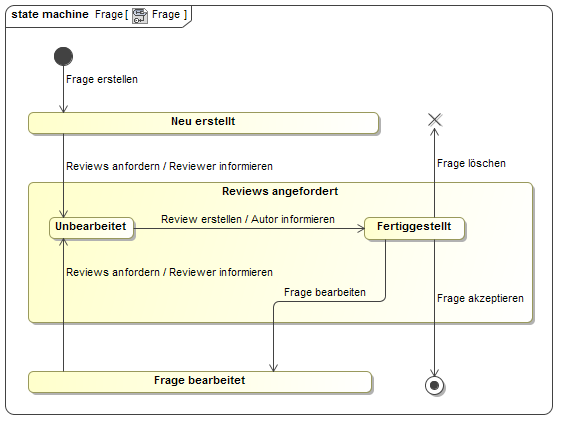
\includegraphics[width=0.8\textwidth]{../Diagramme/State_Machine_Diagram__Frage__Frage.png}
			\label{Zustandsdiagramme}
		\end{frame}
\end{document}